\documentclass[10pt,twocolumn]{article}
\usepackage[letterpaper,margin=0.75in]{geometry}
\usepackage{amsmath,amssymb,graphicx,booktabs,hyperref,microtype}
\setlength{\columnsep}{0.24in}
\hypersetup{colorlinks=true,urlcolor=blue,citecolor=blue,linkcolor=blue}
\title{The Computational Organization of MoE Modularity\\
\large Learning history, property transport, and predictive cooperation}
\author{Research argument draft}
\date{29 October 2026}
\begin{document}
\maketitle
\begin{abstract}
Training MoE models for selective execution raises a scientific question about how expert functions divide computation.
Across six mature public checkpoints in two lineages, we show that selectability can improve while shared dependence grows at similar intact quality.
Among four architecture-matched paths, the same 40 correctly answered questions require routed and shared computation jointly in 8--24 cases.
Source, realized-route and message interventions identify the functions carrying a low-budget likelihood advantage, while showing how unchanged partners and actual messages acquire value through their computational context.
Local geometric correction leaves most message-replay cost intact.
A second lineage reveals an opposite native trend: budget sensitivity increases while the transported expert bank improves restricted likelihood in a common receiver, with backbone changes opposing that improvement.
Gain and shared-path interventions make these separations constructive.
Sixteen calibrated response gains produce a budget benefit in OLMoE; in EMO they increase shared dependence but worsen restricted quality, while the routed bank's advantage survives shared removal.
Together, these results characterize MoE modularity as a learned organization of selectable functions, response interfaces and cooperative use, with different boundaries for a property carrier and reusable computation.
Probability quality and accuracy are reported separately.
\end{abstract}

\section{What organization does modularity learn?}
Sparse MoE models offer a compelling route to scalable, adaptable computation: a large bank of experts can serve different inputs through small active subsets.
Training objectives can go further and make document-level expert pools useful for deployment~\cite{emo}.
Understanding what these objectives organize is central to the scientific promise of MoE: how tasks are divided, which functions carry transferable properties, and which computations can be reused across learning histories.

Our central finding is that these questions have different answers within the same mature systems.
At similar intact quality, a model with better selective execution relies more heavily on shared computation.
The routed-function package carries a low-budget predictive advantage, while its unchanged shared partner becomes more necessary in the common receiver.
Realized messages retain value through their pairing with the surrounding computation.
Thus, learning organizes both a selectable function bank and the relationships through which that bank supports prediction.

The paper develops this finding through a connected intervention sequence.
Native histories establish the change in computational division.
Source crosses identify the carrier of a useful property and the changing role of its partner.
Realized-route and message interventions identify the execution paths supporting these effects.
A second mature lineage demonstrates why native deployment curves alone can miss a transportable component property.
The resulting account links selective deployment to the learned production and use of expert computation.

\section{Objects, interventions, and evidence}
We study four public mature paths from the EMO release~\cite{emo}: a standard pre-annealing parent $P$, standard annealing $A$, EMO annealing $B$, and full-course EMO $F$.
These architecture-matched public paths provide mature endpoints with documented training histories.
Let $D$ denote backbone, attention and readout, $G$ the gate parameters, $R$ the routed expert functions, and $S$ the always-active shared functions.
An $R/S$ intervention covers the corresponding function suites in all 16 layers, defining the unit of the present comparison.

For an intact loss $L$, native language-model selection uses each model's expert pool derived from the first 128 observed input tokens, and scores subsequent targets alongside fixed random pools of the same size.
Property-transport experiments instead use a common parent pool derived from separate task calibration, preserving the selector across all compared sources.
We measure property transport by changing a parameter source while holding a common receiver fixed.
We measure a function's predictive role by its removal effect in the specified system.
These measurements connect deployment behavior, parameter sources, and predictive roles.

Gate parameters held fixed do not imply realized routing held fixed: changed expert outputs can change later hidden states and gate outputs.
We therefore capture actual gate logits before the common pool mask and replay them while preserving the original softmax, top-$k$, multiplication, and accumulation program.
This clamps both support and weights.
If $z$ denotes a replayed trajectory, the shared role in that condition is
\begin{equation}
\Delta_S(R,z)=L(D_P,G_P,R,0;z)-L(D_P,G_P,R,S_P;z).
\end{equation}
Other responses remain endogenous.
The source and trajectory crosses identify controlled effects in this receiver.

Language-model measurements use 64 windows and 20 file clusters.
The initial task panel contains 128 biology and mathematics questions.
The route experiment adds a fixed 440-question panel: eight questions in each of the other 55 MMLU subjects, with separate validation calibration.
The panels use different calibration sample counts, so between-panel magnitude differences cannot be assigned solely to task content.
We report answer-token NLL, choice CE, accuracy, and output KL separately.
Confidence intervals are paired input resampling intervals conditional on the models; they are not training-seed intervals.

\section{Three results and their connection}
\subsection{Selection improves while shared dependence grows}
The late- and full-course EMO endpoints $B/F$ have intact text NLL $2.6218/2.6212$ and identical task raw accuracy $39.06\%$.
Yet $F$ has lower selected-pool damage, while removing shared computation adds $1.8509$ more text NLL damage than in $B$ (95\% CI $[1.3311,2.3010]$).
The corresponding task answer-NLL difference is $5.3112$; the raw-accuracy damage difference remains unresolved.
Random-pool controls show that general robustness and useful selection coexist.
Selectability and cooperation increase together in these endpoints (Figure~\ref{fig:native}). On the previously specified set of 40 questions answered correctly by all four endpoints, both suites are jointly necessary in 8/10/20/24 cases for P/A/B/F. These are selected-set counts, reported alongside the full panel without population confidence claims.

\begin{figure*}[t]
\centering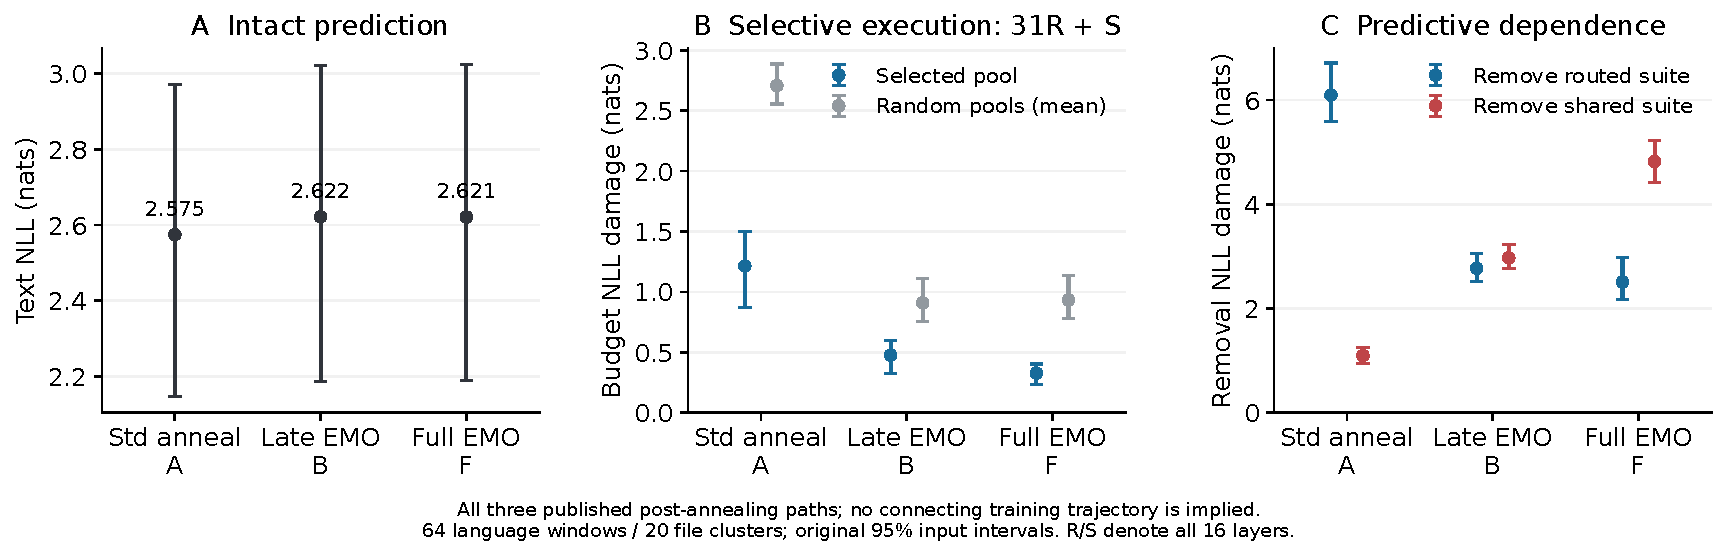
\includegraphics[width=\textwidth]{figures/01_selection_and_dependence.pdf}
\caption{Computational division at similar intact quality. A--C show all three post-annealing paths, selected/random pool damage and routed/shared removal effects with original paired file-cluster intervals. D follows the same 40 questions answered correctly by all four endpoints: joint necessity counts are 8/10/20/24 for P/A/B/F. D reports selected-set counts, with no population interval. Sources: E162/E163.}
\label{fig:native}
\end{figure*}

\subsection{A property carrier also changes the role of an unchanged partner}
In the common $P$ receiver, replacing $R_P$ by $R_B$ transfers a low-budget answer-NLL advantage on the original panel, whereas replacing shared functions alone does not transfer the same property.
The routed source carries a specific operating advantage: original-panel low-budget NLL decreases $0.1882$, while full NLL increases $0.0802$. Intact quality therefore depends on a broader assembly than the transferred property.
Holding $S_P$ fixed and changing $R$ increases its removal effect by $0.3386$.
The function package that carries a useful operating property and the native necessary partner must therefore be identified separately.

The larger subject panel strengthens this statement and locates its runtime implementation (Figure~\ref{fig:routes}).
The natural low-budget NLL advantage is $0.4207$ ($[0.3221,0.5234]$).
At fixed $P/B$ routes, the routed-function source effect remains an improvement of $0.2937/0.3824$, while the unchanged shared suite's removal cost increases $0.2891/0.1840$; all four intervals exclude zero.
Routing still matters: the $B$ trajectory improves $R_B$ by a further $0.1270$, and the function--trajectory interaction is $-0.0887$ ($[-0.1242,-0.0500]$).
Routed-function responses preserve the advantage under fixed execution, and their interaction with the trajectory further shapes its size.

Under natural routing, the choice CE advantage is $1.1386$ ($[0.8431,1.4676]$), but the raw accuracy difference is $+1.14$ percentage points ($[-2.27,4.55]$).
The full-regime role and low-budget property establish two parts of the organization; the same-budget shared intervention below tests their causal connection.

\begin{figure*}[t]
\centering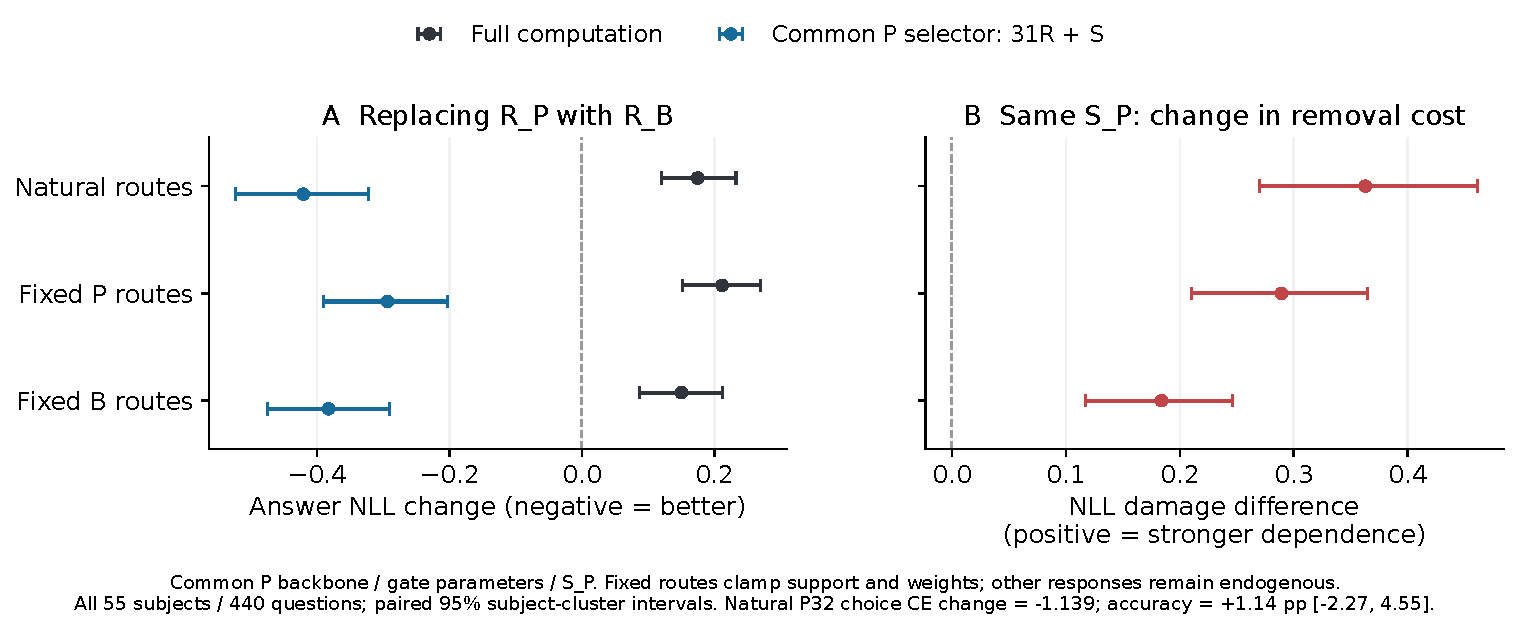
\includegraphics[width=\textwidth]{figures/02_property_and_partner_under_fixed_routes.pdf}
\caption{Two effects survive realized-route fixation on all 55 subjects. Left: changing only the routed function source improves low-budget likelihood while worsening full likelihood. Right: the same change increases the removal cost of unchanged shared functions. The actual support and weights are clamped; other response paths remain endogenous. Original subject-cluster intervals and accuracy boundary are shown. Source: E164.}
\label{fig:routes}
\end{figure*}

\subsection{Realized messages retain context-dependent value}
Function identity leaves production and use entangled.
We therefore fix shared functions and cross their actual messages between routed-function contexts on the same input.
Foreign messages have an average answer-NLL cost of $0.2605$ relative to their original pairing.
Correcting the consumer's clean norm and residual projection reduces this cost only to $0.2459$ ($[0.2096,0.2819]$).
The improvement is $0.0146$ ($[0.0050,0.0250]$), concentrated in biology rather than mathematics; choice CE and accuracy do not show equivalent recovery (Figure~\ref{fig:messages}).
The tested local scalar interface does not account for most of the prediction mismatch.
The residual prediction cost motivates studying the message structure and receiving computation together.

\begin{figure*}[t]
\centering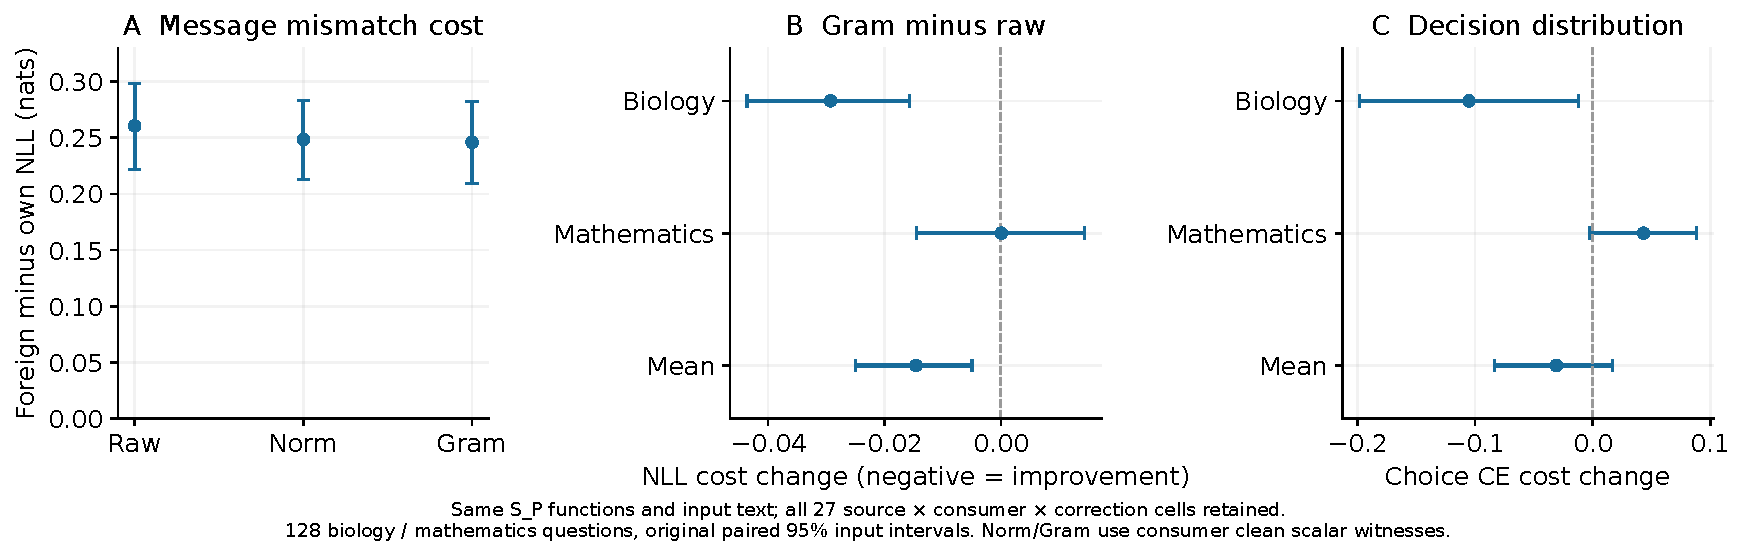
\includegraphics[width=\textwidth]{figures/03_actual_message_reuse.pdf}
\caption{Actual-message reuse after local correction. All 27 source--consumer--correction cells are retained in the underlying results. Norm and Gram corrections give modest answer-NLL recovery; the subject and choice-CE panels retain the heterogeneous outcomes. Source: E163.}
\label{fig:messages}
\end{figure*}

\section{Native curves can conceal transportable properties}
We evaluate OLMoE's public 5.033T checkpoint and its ordinary 100B annealing endpoint~\cite{olmoe}, crossing backbone, gate and expert sources under full computation and one fixed parent-calibrated pool of 16/64 experts.
Its 64 routed experts and absence of an always-active shared expert extend the source--context analysis to a different architecture.
All 26 predeclared conditions cover the same 55 subjects and 440 question texts, re-encoded by the OLMoE tokenizer.

After annealing, native restricted NLL damage increases by $0.1050$ ($[0.0021,0.2059]$).
Yet the annealed expert bank improves restricted NLL in the common parent receiver by $0.2230$ at fixed parent routes ($[0.1459,0.3021]$), with a choice-CE improvement of $0.4876$ ($[0.0844,0.8817]$).
Backbone changes oppose this property: at fixed parent gate parameters, changing only the backbone increases restricted NLL by $0.3575$ with the parent bank and $0.3176$ with the annealed bank (Figure~\ref{fig:lineage}).
Native deployment curves therefore need not monotonically track a component's property in a controlled receiver.

The restricted regime is severely impaired: raw accuracy is only $22.05/21.14\%$ compared to intact $43.64/43.18\%$.
This intervention identifies a probability-quality property in a severely impaired restricted regime.
The cross-lineage result extends the separation between a property carrier and its native operating context.
Different tokenizers also preclude directly subtracting the two lineages' absolute NLL values.

\begin{figure*}[t]
\centering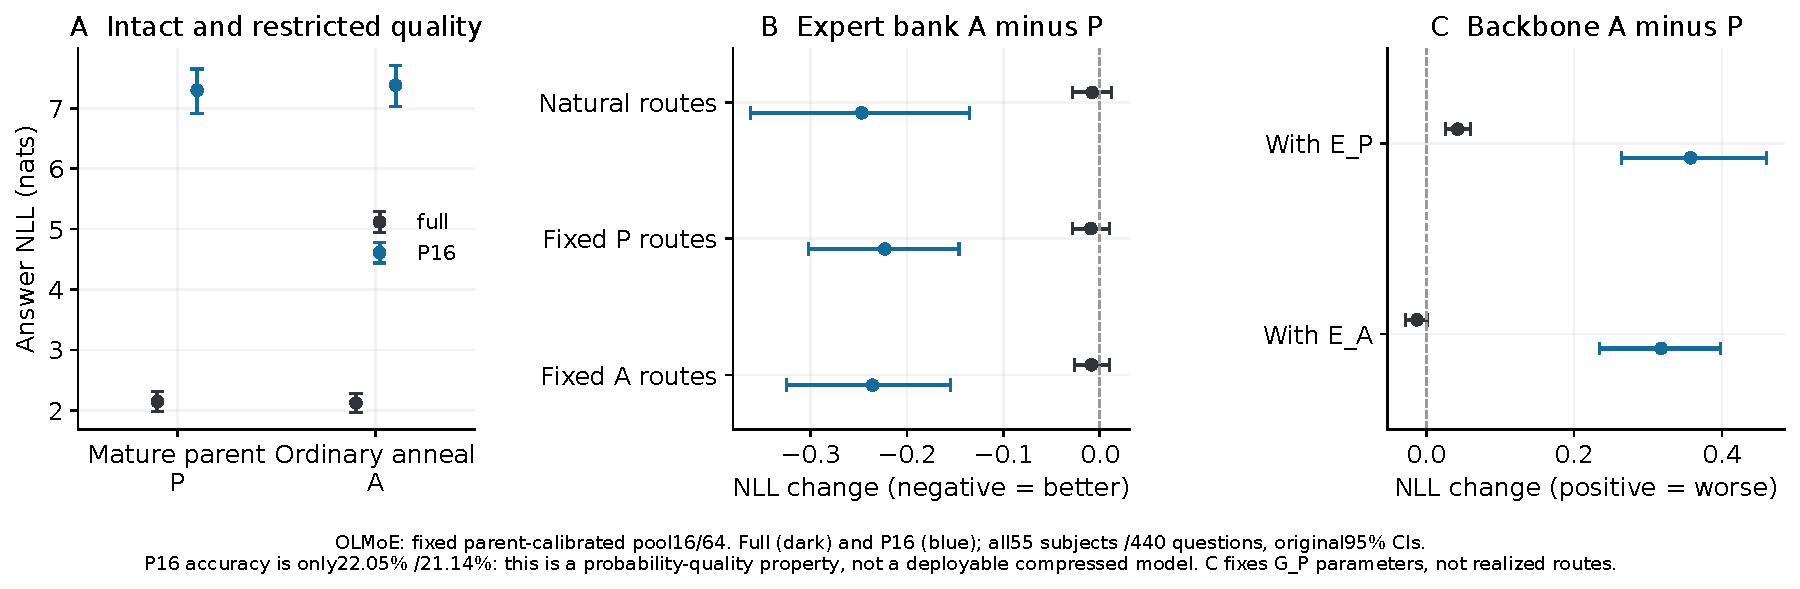
\includegraphics[width=\textwidth]{figures/04_native_trends_and_transport.pdf}
\caption{Native curves can conceal component properties. OLMoE expert-source changes improve restricted likelihood in the common parent receiver, including after realized-route fixation, while backbone changes oppose the improvement. Intact and restricted quality remain separate. The native restricted model is severely damaged; all source corners and accuracy boundaries are retained. Source: E165.}
\label{fig:lineage}
\end{figure*}

\section{Interventions separate properties and partner dependence}
The separation between a deployment property and its underlying computation also allows a constructive test.
We match donor routed-response energy on native full-parent calibration inputs using one fixed positive scalar per layer, then apply these 16 gains to the parent's routed functions.
Both the original parent functions and their shared partner are retained; actual routes are held fixed within each operating policy.
The coefficients use full-computation calibration responses and no predictive-loss fitting or restricted-policy tuning.

In OLMoE, the resulting gains range from $0.931$ to $1.000$.
The gain-adjusted parent improves restricted answer NLL by $0.276$ ($[0.241,0.315]$), compared to $0.223$ ($[0.140,0.308]$) from the annealed expert bank.
Choice CE improves $0.697$ ($[0.467,0.915]$), compared to $0.488$ ($[0.069,0.920]$) from the bank.
The gain-adjusted model remains close to full parent prediction: full answer NLL changes $+0.0042$ and first-answer vocabulary KL is $0.0037$, versus $0.0831$ for the donor bank.
Descriptively, gains improve restricted NLL in 54 of the 55 subjects, and the bank improves it in 45; all subjects remain in the analysis.

These results provide an alternative functional implementation of the operating property.
An energy-calibrated parent and an annealed bank can both improve restricted execution while making different changes to full prediction.
The property is consequently understood through its response interface and operating context, alongside the parameter package that carries it.
This connects the native reversal in Figure~\ref{fig:lineage} to a controllable factor in the computational organization.

The EMO cross reveals a complementary separation.
Gain calibration increases the full-regime removal cost of unchanged shared functions by $0.863$ ($[0.760,0.970]$), compared to $0.289$ ($[0.210,0.371]$) from the donor bank.
Yet gains worsen restricted answer NLL by $0.394$ ($[0.237,0.594]$), while the bank improves it by $0.294$ ($[0.204,0.385]$).
The direct gain-minus-bank difference is $+0.688$ ($[0.520,0.898]$).
Choice CE also changes in opposite directions: gains worsen it by $0.919$, while the bank improves it by $0.725$.
Full-regime NLL changes are $+0.153/+0.212$ for gains/bank, so the gain construction has less intact-NLL damage while failing to reproduce the restricted advantage.

The same-budget shared intervention connects the property and cooperation questions directly.
With shared outputs zeroed, the routed bank still improves restricted answer NLL by $0.356$ ($[0.148,0.553]$), compared to $0.294$ with shared computation active.
The shared pathway remains useful for prediction: its absolute removal costs are $1.333/1.271$ for parent/donor in this policy.
Thus, the routed-source NLL advantage survives removal of that online pathway, while increased full-regime dependence can be produced without the advantage (Figure~\ref{fig:gains}).

\begin{figure*}[t]
\centering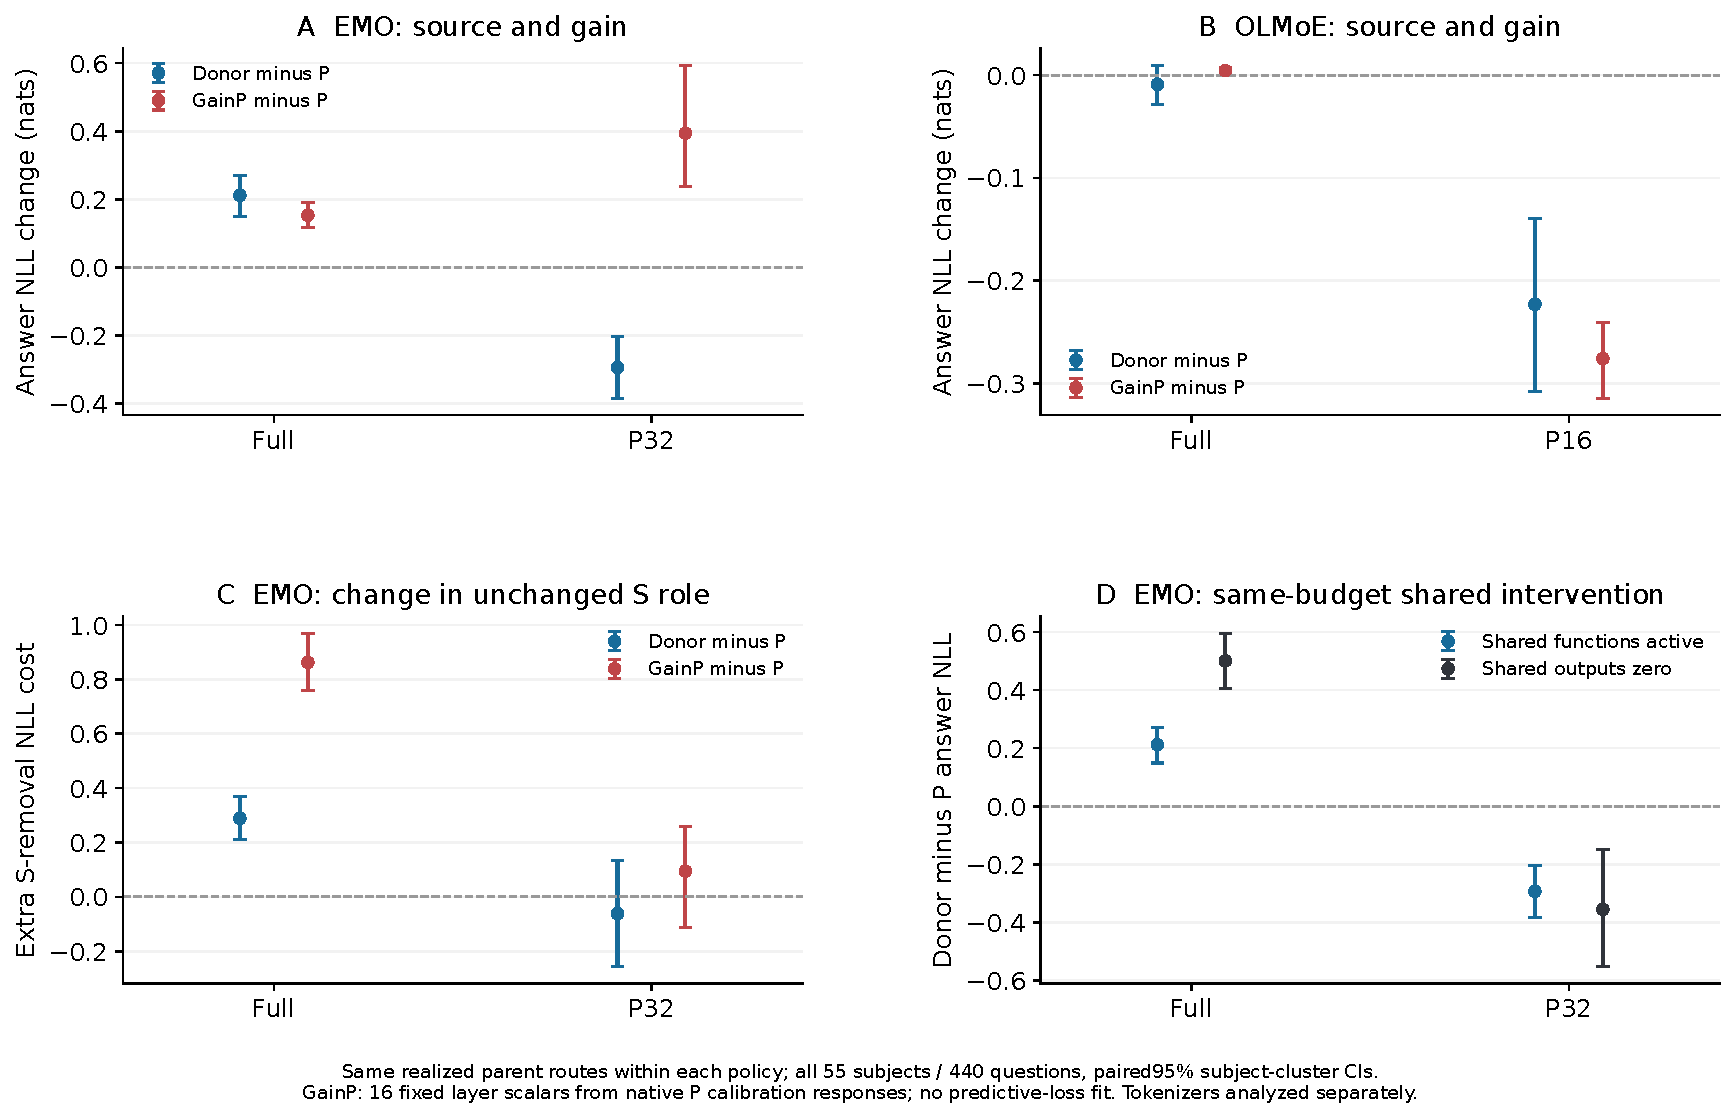
\includegraphics[width=\textwidth]{figures/05_gain_and_partner_interventions.pdf}
\caption{Interventions connect the computational-organization account. A--B: gain calibration produces a restricted-likelihood benefit in OLMoE, but has the opposite effect to the transported bank in EMO. C: gains nevertheless increase dependence on unchanged shared functions in EMO's full regime. D: the bank's restricted NLL advantage survives shared-output removal. Actual parent support and weights are fixed within each policy; all 55 subjects are retained. Source: E166.}
\label{fig:gains}
\end{figure*}

These constructions separate an operating property from the cooperation that accompanies it in a mature model.
They identify response gains as a controllable interface factor and show why the same factor need not reproduce the organization learned by another history.
Combined with the source, route and message interventions, they explain why selective deployment, the carrier of a property, and reusable computation can have different boundaries.

\section{Connection to MoE and interpretability research}
\paragraph{Training and deployment.}
EMO trains document-level selectable expert pools~\cite{emo}; interaction-aware pruning preserves cooperative structure~\cite{hope}; condensation retains effective shared computation~\cite{cdmoe}.
DeepSeekMoE couples fine-grained expert combinations with shared experts and evaluates routed exclusion, shared replacement, and reduced activation~\cite{deepseekmoe}.
These works establish the value of selective and shared computation.
Our intervention sequence explains how mature learning histories realize these properties through changing function sources, partner roles, and message use.

\paragraph{Representation and computational reuse.}
Spectral decoupling organizes common parameter and gradient subspaces~\cite{sdmoe}; basic--refinement attribution measures shared/routed contributions~\cite{basic}; stitching tests functional-feature transport after alignment~\cite{stitch,howstitch,invariance}.
We connect these perspectives by following a deployment property from its source functions through realized routing to the messages used by its partners.
This yields a concrete account of why a selectable component's useful property and its computational reuse can have different boundaries.

\section{Evidence scope and implications}
The primary objects are mature public learning paths and interventions on all-layer function suites.
Input confidence intervals condition on these models and calibration data; independent initialization populations and formation trajectories remain open.
The complete source grids, accuracy results, failed attempts, numerical programs and raw inputs are preserved, with JSON paths and SHA256 for every plotted estimate.
Native identity replays, causal-prefix checks, source read-only checks and independent formula recomputation validate the measurement program.

The scientific implication is that the division of computation in MoE is expressed through both functions and their learned use relationships.
Selective deployment, a transportable property, and reusable actual computation identify complementary parts of that organization.
Understanding their relationship provides a basis for studying how computational responsibilities form, repeat across histories, and support model composition.

\begin{thebibliography}{99}
\bibitem{emo} R. Wang et al. \emph{EMO: Pretraining Mixture of Experts for Emergent Modularity}. 2026. \url{https://arxiv.org/abs/2605.06663}.
\bibitem{hope} A. M. Tseng et al. \emph{Higher-order pruning of experts in mixture-of-experts language models}. arXiv:2609.18916v3, 2026.
\bibitem{cdmoe} M. Cao et al. \emph{Condense, Don't Just Prune}. TMLR, 2025; reading version arXiv:2412.00069v3.
\bibitem{sdmoe} R. Huang et al. \emph{SD-MoE: Spectral Decomposition for Effective Expert Specialization}. ICML, 2026.
\bibitem{basic} J. Li et al. \emph{Decoding Knowledge Attribution in Mixture-of-Experts: A Framework of Basic-Refinement Collaboration and Efficiency Analysis}. ACL, 2025.
\bibitem{stitch} \emph{Transferring Linear Features Across Language Models With Model Stitching}. NeurIPS, 2025.
\bibitem{howstitch} \emph{How Not to Stitch Representations to Measure Similarity}. AAAI, 2025.
\bibitem{invariance} \emph{Grounding Functional Similarity by Invariance-Aware Model Stitching}. ICML, 2026; reading version arXiv:2505.20142v2.
\bibitem{deepseekmoe} D. Dai et al. \emph{DeepSeekMoE: Towards Ultimate Expert Specialization in Mixture-of-Experts Language Models}. arXiv:2401.06066v1, 2024.
\bibitem{olmoe} N. Muennighoff et al. \emph{OLMoE: Open Mixture-of-Experts Language Models}. ICLR, 2025. \url{https://huggingface.co/allenai/OLMoE-1B-7B-0924}.
\bibitem{massive} M. Sun et al. \emph{Massive Activations in Large Language Models}. COLM, 2024; arXiv:2402.17762v2.
\bibitem{super} Z. Su et al. \emph{Unveiling Super Experts in Mixture-of-Experts Large Language Models}. ICLR, 2026.
\bibitem{melayer} Z. Shi et al. \emph{A Single Layer to Explain Them All: Understanding Massive Activations in Large Language Models}. ICML, 2026.
\bibitem{aoe} A. Lv et al. \emph{Autonomy-of-Experts Models}. ICML, 2025.
\end{thebibliography}

\appendix
\section{Intervention and reproduction details}
\paragraph{Mature paths.}
The EMO release provides four 16-layer, 128-expert checkpoints with 127 routed experts and one always-active shared expert; each token activates seven routed experts plus the shared expert.
The parent is \texttt{StdMoE\_1b14b\_1T\_Preanneal}; standard and EMO annealing produce \texttt{StdMoE\_1b14b\_1T} and \texttt{StdMoE\_1b14b\_1T\_EmoAnnealed}; the full-course path is \texttt{Emo\_1b14b\_1T}.
The paths use 1T pretraining and 50B annealing tokens.
OLMoE uses 16 layers, 64 routed experts, top-8 activation and no shared expert.
Its comparison follows the public step-1,200,000 checkpoint at 5.033T tokens to the ordinary 100B annealing endpoint.
Exact public revisions, file SHA256, native code, model fingerprints, configurations and raw inputs are registered in the repository manifests.

\paragraph{Source crosses and runtime fixation.}
In the EMO common receiver, $D_P$, $G_P$ and $S_P$ are retained while the routed functions in every layer come from $P$ or $B$.
The $P/B$ route origins refer to these two receiver computations.
For each candidate continuation and policy, gate logits are captured before the pool mask, then replayed with the original softmax, top-$k$, gate multiplication and accumulation.
The routed support and weights therefore agree across the compared function sources, while the downstream hidden states and shared responses evolve naturally.
The same-budget shared intervention zeros shared outputs under the trajectory captured with shared computation active.
Its paired source interaction measures how the shared pathway contributes in that execution condition.

\paragraph{Inputs and selection.}
The broader panel contains all 55 MMLU subjects outside the original biology/mathematics pair, with eight held-out questions and eight validation calibration texts per subject.
Five fixed development examples provide the few-shot prefix.
The text population is shared between the two lineages and encoded separately by their native tokenizers, with no truncation.
For source transport and gain experiments, a parent-calibrated sequential greedy selector fixes the task pool in every consumer: 31 routed experts plus $S$ for EMO and 16/64 experts for OLMoE.
The native language-model experiment uses each endpoint's own 128-token context-prefix selector instead, evaluating only subsequent targets. Its random-pool controls and both pool/full-denominator programs are retained in the complete results.
Pool masking precedes the native softmax; the original top-$k$ width and normalization convention are retained.
Native random pools provide a separate selection-value control.

\paragraph{Gain comparison.}
On native full-$P$ calibration trajectories, the parent and donor routed suites are evaluated on the same layer inputs with the same parent gate.
EMO shared outputs are excluded from this energy measurement.
For layer $l$, the fixed coefficient is
\begin{equation}
 a_l=\sqrt{\frac{\sum_{\mathrm{cal}}\lVert r_{D,l}\rVert_2^2}
                         {\sum_{\mathrm{cal}}\lVert r_{P,l}\rVert_2^2}}.
\end{equation}
The 16 coefficients are common to every expert, subject and execution policy in that lineage.
Calibration texts include the original correct continuations; the procedure fits activation energy and uses no predictive-loss optimization or held-out tuning.
Each routed-expert output is multiplied in FP32 and cast back to BF16 before the original gate multiplication and summation; shared outputs retain the native program.
Full and restricted policies are evaluated for parent, donor and gain-adjusted parent; EMO additionally crosses each with shared-output removal.

\paragraph{Statistics and numerical program.}
Candidate log likelihoods sum all answer-token scores.
Answer-token NLL, normalized four-choice CE, raw accuracy, per-character accuracy and first-answer full-vocabulary KL are reported separately.
The 55-subject analysis uses equally weighted paired subject clusters, 2,000 bootstrap draws and frozen seeds; tokenizers are analyzed separately. Replayed source conditions have identical point estimates; intervals retain each experiment's predeclared draws and their small Monte Carlo differences.
KL uses FP32 products and FP64 reduction.
Canonical parameter/buffer fingerprints, exact old-condition LL/KL replays, causal-prefix and permutation controls, unit/zero gain identities and terminal source checks preserve the native interface.
A separate coefficient-vector/logaddexp program recomputes the score contrasts and intervals.
The reproduction entrypoint executes statistics, verification and plots from durable raw arrays without a model forward.

\end{document}
